\documentclass[border=4pt]{standalone}

\usepackage{amsmath}
\usepackage{tikz}
\usepackage{mathdots}
\usepackage{yhmath}
\usepackage{cancel}
\usepackage{color}
\usepackage{siunitx}
\usepackage{array}
\usepackage{multirow}
\usepackage{amssymb}
\usepackage{gensymb}
\usepackage{tabularx}
\usepackage{booktabs}
\usetikzlibrary{fadings}
\usetikzlibrary{patterns}


\begin{document}
 
     

\tikzset{every picture/.style={line width=0.75pt}} %set default line width to 0.75pt        

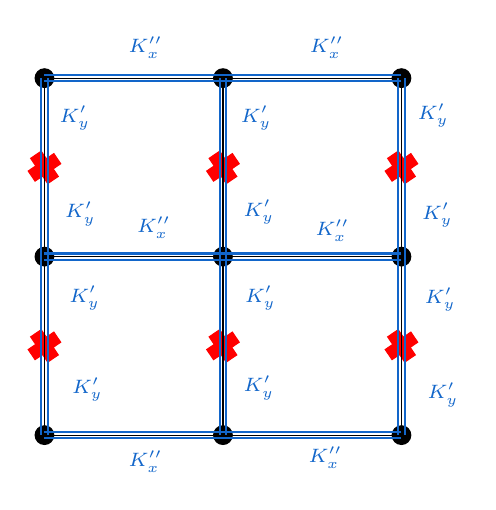
\begin{tikzpicture}[x=0.75pt,y=0.75pt,yscale=-1,xscale=1]
%uncomment if require: \path (0,300); %set diagram left start at 0, and has height of 300

%Shape: Circle [id:dp7535807123858111] 
\draw  [color={rgb, 255:red, 0; green, 0; blue, 0 }  ,draw opacity=1 ][fill={rgb, 255:red, 0; green, 0; blue, 0 }  ,fill opacity=1 ] (153.5,62) .. controls (153.5,59.51) and (155.51,57.5) .. (158,57.5) .. controls (160.49,57.5) and (162.5,59.51) .. (162.5,62) .. controls (162.5,64.49) and (160.49,66.5) .. (158,66.5) .. controls (155.51,66.5) and (153.5,64.49) .. (153.5,62) -- cycle ;
%Shape: Circle [id:dp4189176698661261] 
\draw  [color={rgb, 255:red, 0; green, 0; blue, 0 }  ,draw opacity=1 ][fill={rgb, 255:red, 0; green, 0; blue, 0 }  ,fill opacity=1 ] (153.5,148) .. controls (153.5,145.51) and (155.51,143.5) .. (158,143.5) .. controls (160.49,143.5) and (162.5,145.51) .. (162.5,148) .. controls (162.5,150.49) and (160.49,152.5) .. (158,152.5) .. controls (155.51,152.5) and (153.5,150.49) .. (153.5,148) -- cycle ;
%Shape: Circle [id:dp3260567741443583] 
\draw  [color={rgb, 255:red, 0; green, 0; blue, 0 }  ,draw opacity=1 ][fill={rgb, 255:red, 0; green, 0; blue, 0 }  ,fill opacity=1 ] (153.5,234) .. controls (153.5,231.51) and (155.51,229.5) .. (158,229.5) .. controls (160.49,229.5) and (162.5,231.51) .. (162.5,234) .. controls (162.5,236.49) and (160.49,238.5) .. (158,238.5) .. controls (155.51,238.5) and (153.5,236.49) .. (153.5,234) -- cycle ;
%Shape: Circle [id:dp15481003747045263] 
\draw  [color={rgb, 255:red, 0; green, 0; blue, 0 }  ,draw opacity=1 ][fill={rgb, 255:red, 0; green, 0; blue, 0 }  ,fill opacity=1 ] (239.5,234) .. controls (239.5,231.51) and (241.51,229.5) .. (244,229.5) .. controls (246.49,229.5) and (248.5,231.51) .. (248.5,234) .. controls (248.5,236.49) and (246.49,238.5) .. (244,238.5) .. controls (241.51,238.5) and (239.5,236.49) .. (239.5,234) -- cycle ;
%Shape: Circle [id:dp21436325902114617] 
\draw  [color={rgb, 255:red, 0; green, 0; blue, 0 }  ,draw opacity=1 ][fill={rgb, 255:red, 0; green, 0; blue, 0 }  ,fill opacity=1 ] (239.5,148) .. controls (239.5,145.51) and (241.51,143.5) .. (244,143.5) .. controls (246.49,143.5) and (248.5,145.51) .. (248.5,148) .. controls (248.5,150.49) and (246.49,152.5) .. (244,152.5) .. controls (241.51,152.5) and (239.5,150.49) .. (239.5,148) -- cycle ;
%Shape: Circle [id:dp31587103984398235] 
\draw  [color={rgb, 255:red, 0; green, 0; blue, 0 }  ,draw opacity=1 ][fill={rgb, 255:red, 0; green, 0; blue, 0 }  ,fill opacity=1 ] (239.5,62) .. controls (239.5,59.51) and (241.51,57.5) .. (244,57.5) .. controls (246.49,57.5) and (248.5,59.51) .. (248.5,62) .. controls (248.5,64.49) and (246.49,66.5) .. (244,66.5) .. controls (241.51,66.5) and (239.5,64.49) .. (239.5,62) -- cycle ;
%Shape: Cross [id:dp44121424098628004] 
\draw  [color={rgb, 255:red, 255; green, 0; blue, 0 }  ,draw opacity=1 ][fill={rgb, 255:red, 255; green, 0; blue, 0 }  ,fill opacity=1 ] (162.53,98.38) -- (165.82,103.24) -- (162.18,105.71) -- (164.65,109.35) -- (159.58,112.79) -- (157.11,109.15) -- (153.47,111.62) -- (150.18,106.76) -- (153.82,104.29) -- (151.35,100.65) -- (156.42,97.21) -- (158.89,100.85) -- cycle ;
%Shape: Cross [id:dp746180121869644] 
\draw  [color={rgb, 255:red, 255; green, 0; blue, 0 }  ,draw opacity=1 ][fill={rgb, 255:red, 255; green, 0; blue, 0 }  ,fill opacity=1 ] (334.53,98.38) -- (337.82,103.24) -- (334.18,105.71) -- (336.65,109.35) -- (331.58,112.79) -- (329.11,109.15) -- (325.47,111.62) -- (322.18,106.76) -- (325.82,104.29) -- (323.35,100.65) -- (328.42,97.21) -- (330.89,100.85) -- cycle ;
%Shape: Cross [id:dp5828407747695723] 
\draw  [color={rgb, 255:red, 255; green, 0; blue, 0 }  ,draw opacity=1 ][fill={rgb, 255:red, 255; green, 0; blue, 0 }  ,fill opacity=1 ] (162.53,184.38) -- (165.82,189.24) -- (162.18,191.71) -- (164.65,195.35) -- (159.58,198.79) -- (157.11,195.15) -- (153.47,197.62) -- (150.18,192.76) -- (153.82,190.29) -- (151.35,186.65) -- (156.42,183.21) -- (158.89,186.85) -- cycle ;
%Shape: Cross [id:dp33669072342309314] 
\draw  [color={rgb, 255:red, 255; green, 0; blue, 0 }  ,draw opacity=1 ][fill={rgb, 255:red, 255; green, 0; blue, 0 }  ,fill opacity=1 ] (248.53,98.38) -- (251.82,103.24) -- (248.18,105.71) -- (250.65,109.35) -- (245.58,112.79) -- (243.11,109.15) -- (239.47,111.62) -- (236.18,106.76) -- (239.82,104.29) -- (237.35,100.65) -- (242.42,97.21) -- (244.89,100.85) -- cycle ;
%Shape: Cross [id:dp7897100484845923] 
\draw  [color={rgb, 255:red, 255; green, 0; blue, 0 }  ,draw opacity=1 ][fill={rgb, 255:red, 255; green, 0; blue, 0 }  ,fill opacity=1 ] (248.53,184.38) -- (251.82,189.24) -- (248.18,191.71) -- (250.65,195.35) -- (245.58,198.79) -- (243.11,195.15) -- (239.47,197.62) -- (236.18,192.76) -- (239.82,190.29) -- (237.35,186.65) -- (242.42,183.21) -- (244.89,186.85) -- cycle ;
%Shape: Cross [id:dp5746061358055936] 
\draw  [color={rgb, 255:red, 255; green, 0; blue, 0 }  ,draw opacity=1 ][fill={rgb, 255:red, 255; green, 0; blue, 0 }  ,fill opacity=1 ] (334.53,184.38) -- (337.82,189.24) -- (334.18,191.71) -- (336.65,195.35) -- (331.58,198.79) -- (329.11,195.15) -- (325.47,197.62) -- (322.18,192.76) -- (325.82,190.29) -- (323.35,186.65) -- (328.42,183.21) -- (330.89,186.85) -- cycle ;
%Shape: Circle [id:dp562238023293715] 
\draw  [color={rgb, 255:red, 0; green, 0; blue, 0 }  ,draw opacity=1 ][fill={rgb, 255:red, 0; green, 0; blue, 0 }  ,fill opacity=1 ] (325.5,62) .. controls (325.5,59.51) and (327.51,57.5) .. (330,57.5) .. controls (332.49,57.5) and (334.5,59.51) .. (334.5,62) .. controls (334.5,64.49) and (332.49,66.5) .. (330,66.5) .. controls (327.51,66.5) and (325.5,64.49) .. (325.5,62) -- cycle ;
%Shape: Circle [id:dp37972492666492985] 
\draw  [color={rgb, 255:red, 0; green, 0; blue, 0 }  ,draw opacity=1 ][fill={rgb, 255:red, 0; green, 0; blue, 0 }  ,fill opacity=1 ] (325.5,148) .. controls (325.5,145.51) and (327.51,143.5) .. (330,143.5) .. controls (332.49,143.5) and (334.5,145.51) .. (334.5,148) .. controls (334.5,150.49) and (332.49,152.5) .. (330,152.5) .. controls (327.51,152.5) and (325.5,150.49) .. (325.5,148) -- cycle ;
%Shape: Circle [id:dp2618781119153002] 
\draw  [color={rgb, 255:red, 0; green, 0; blue, 0 }  ,draw opacity=1 ][fill={rgb, 255:red, 0; green, 0; blue, 0 }  ,fill opacity=1 ] (325.5,234) .. controls (325.5,231.51) and (327.51,229.5) .. (330,229.5) .. controls (332.49,229.5) and (334.5,231.51) .. (334.5,234) .. controls (334.5,236.49) and (332.49,238.5) .. (330,238.5) .. controls (327.51,238.5) and (325.5,236.49) .. (325.5,234) -- cycle ;
%Straight Lines [id:da6831085309890812] 
\draw    (158,62) -- (330,62) ;


%Straight Lines [id:da9575787161844229] 
\draw    (158,234) -- (330,234) ;


%Straight Lines [id:da46285036316992945] 
\draw    (158,148) -- (330,148) ;


%Straight Lines [id:da7786558478958083] 
\draw    (158,234) -- (158,62) ;


%Straight Lines [id:da5817231613959941] 
\draw    (244,234) -- (244,62) ;


%Straight Lines [id:da690167648664719] 
\draw    (330,234) -- (330,62) ;


%Straight Lines [id:da01605982705380149] 
\draw [color={rgb, 255:red, 18; green, 102; blue, 202 }  ,draw opacity=1 ][line width=0.75]    (331.5,62) -- (331.5,234)(328.5,62) -- (328.5,234) ;


%Straight Lines [id:da27264666983355723] 
\draw [color={rgb, 255:red, 18; green, 102; blue, 202 }  ,draw opacity=1 ][line width=0.75]    (245.5,62) -- (245.5,234)(242.5,62) -- (242.5,234) ;


%Straight Lines [id:da027877897402112106] 
\draw [color={rgb, 255:red, 18; green, 102; blue, 202 }  ,draw opacity=1 ][line width=0.75]    (159.5,62) -- (159.5,234)(156.5,62) -- (156.5,234) ;


%Straight Lines [id:da8628697754234955] 
\draw [color={rgb, 255:red, 18; green, 102; blue, 202 }  ,draw opacity=1 ][line width=0.75]    (330,63.5) -- (158,63.5)(330,60.5) -- (158,60.5) ;


%Straight Lines [id:da4478721967493411] 
\draw [color={rgb, 255:red, 18; green, 102; blue, 202 }  ,draw opacity=1 ][line width=0.75]    (330,149.5) -- (158,149.5)(330,146.5) -- (158,146.5) ;


%Straight Lines [id:da40171975125083925] 
\draw [color={rgb, 255:red, 18; green, 102; blue, 202 }  ,draw opacity=1 ][line width=0.75]    (330,235.5) -- (158,235.5)(330,232.5) -- (158,232.5) ;



% Text Node
\draw (172.67,81.33) node  [font=\scriptsize,color={rgb, 255:red, 18; green, 102; blue, 202 }  ,opacity=1 ]  {$K'_{y}$};
% Text Node
\draw (175.33,127.33) node  [font=\scriptsize,color={rgb, 255:red, 18; green, 102; blue, 202 }  ,opacity=1 ]  {$K'_{y}$};
% Text Node
\draw (177.33,168) node  [font=\scriptsize,color={rgb, 255:red, 18; green, 102; blue, 202 }  ,opacity=1 ]  {$K'_{y}$};
% Text Node
\draw (178.67,212) node  [font=\scriptsize,color={rgb, 255:red, 18; green, 102; blue, 202 }  ,opacity=1 ]  {$K'_{y}$};
% Text Node
\draw (345.33,80) node  [font=\scriptsize,color={rgb, 255:red, 18; green, 102; blue, 202 }  ,opacity=1 ]  {$K'_{y}$};
% Text Node
\draw (347.33,128) node  [font=\scriptsize,color={rgb, 255:red, 18; green, 102; blue, 202 }  ,opacity=1 ]  {$K'_{y}$};
% Text Node
\draw (348.67,168.67) node  [font=\scriptsize,color={rgb, 255:red, 18; green, 102; blue, 202 }  ,opacity=1 ]  {$K'_{y}$};
% Text Node
\draw (350,214.67) node  [font=\scriptsize,color={rgb, 255:red, 18; green, 102; blue, 202 }  ,opacity=1 ]  {$K'_{y}$};
% Text Node
\draw (210.67,134) node  [font=\scriptsize,color={rgb, 255:red, 18; green, 102; blue, 202 }  ,opacity=1 ]  {$K''_{x}$};
% Text Node
\draw (296.67,135.33) node  [font=\scriptsize,color={rgb, 255:red, 18; green, 102; blue, 202 }  ,opacity=1 ]  {$K''_{x}$};
% Text Node
\draw (206.67,47.33) node  [font=\scriptsize,color={rgb, 255:red, 18; green, 102; blue, 202 }  ,opacity=1 ]  {$K''_{x}$};
% Text Node
\draw (294,47.33) node  [font=\scriptsize,color={rgb, 255:red, 18; green, 102; blue, 202 }  ,opacity=1 ]  {$K''_{x}$};
% Text Node
\draw (206.67,246.67) node  [font=\scriptsize,color={rgb, 255:red, 18; green, 102; blue, 202 }  ,opacity=1 ]  {$K''_{x}$};
% Text Node
\draw (293.33,244.67) node  [font=\scriptsize,color={rgb, 255:red, 18; green, 102; blue, 202 }  ,opacity=1 ]  {$K''_{x}$};
% Text Node
\draw (261.33,211.33) node  [font=\scriptsize,color={rgb, 255:red, 18; green, 102; blue, 202 }  ,opacity=1 ]  {$K'_{y}$};
% Text Node
\draw (262,168) node  [font=\scriptsize,color={rgb, 255:red, 18; green, 102; blue, 202 }  ,opacity=1 ]  {$K'_{y}$};
% Text Node
\draw (261.33,126.67) node  [font=\scriptsize,color={rgb, 255:red, 18; green, 102; blue, 202 }  ,opacity=1 ]  {$K'_{y}$};
% Text Node
\draw (260,81.33) node  [font=\scriptsize,color={rgb, 255:red, 18; green, 102; blue, 202 }  ,opacity=1 ]  {$K'_{y}$};


\end{tikzpicture}

\end{document}
